\section{Systems A, B, and C under a common protocol}\label{sec:case}

Because the studies reviewed above were evaluated with different samples, references, and metrics, it is hard to say how much of the reported differences comes from the hardware and how much from the way each instrument was tested. To see what a common protocol reveals, we measured three inexpensive instruments side by side, using the same dye solutions, cuvettes, light source, and laboratory reference for all of them.

There were several reasons for choosing these three instruments. Together they represent two of the most widespread routes in the literature: a multispectral sensor chip, the largest hardware family in Table~\ref{tab:valpractice}, and a camera-based grating spectrometer, the approach shared by the smartphone and camera families. All three cost less than \euro{}220, which places them well within the price range of the instruments reviewed. They also illustrate three ways in which a user can obtain such an instrument: building it around an open sensor board (system A), assembling it from a commercial pocket spectroscope and a single-board computer running open software (system B), or buying it ready-made (system C). Finally, the three instruments were available to us through our work on low-cost tools for monitoring water quality, which is the kind of application such devices are intended for.

System A uses an AS7265x multispectral sensor, system B a Raspberry Pi camera behind a pocket spectroscope, and system C a Little Garden webcam spectrometer. For each, we evaluated absorbance agreement with the reference, repeatability, calibration size, and cost.

\subsection{Materials and methods}\label{sec2}

The reference instrument was a single-beam Genesys~30 spectrophotometer (Thermo Fisher Scientific; 325--1100~nm). Its specified bandwidth is 5~nm, its wavelength accuracy $\pm$2~nm, and its photometric accuracy $\pm$0.002 absorbance units between 0 and 0.3 and 0.5\% of the reading between 0.301 and 2.5.\citep{thermoGenesys30}

\subsubsection{Systems A, B, and C}\label{subsec2.1}

Figure~\ref{fig:systems} shows the three systems.

\begin{figure}[!htbp]
\centering
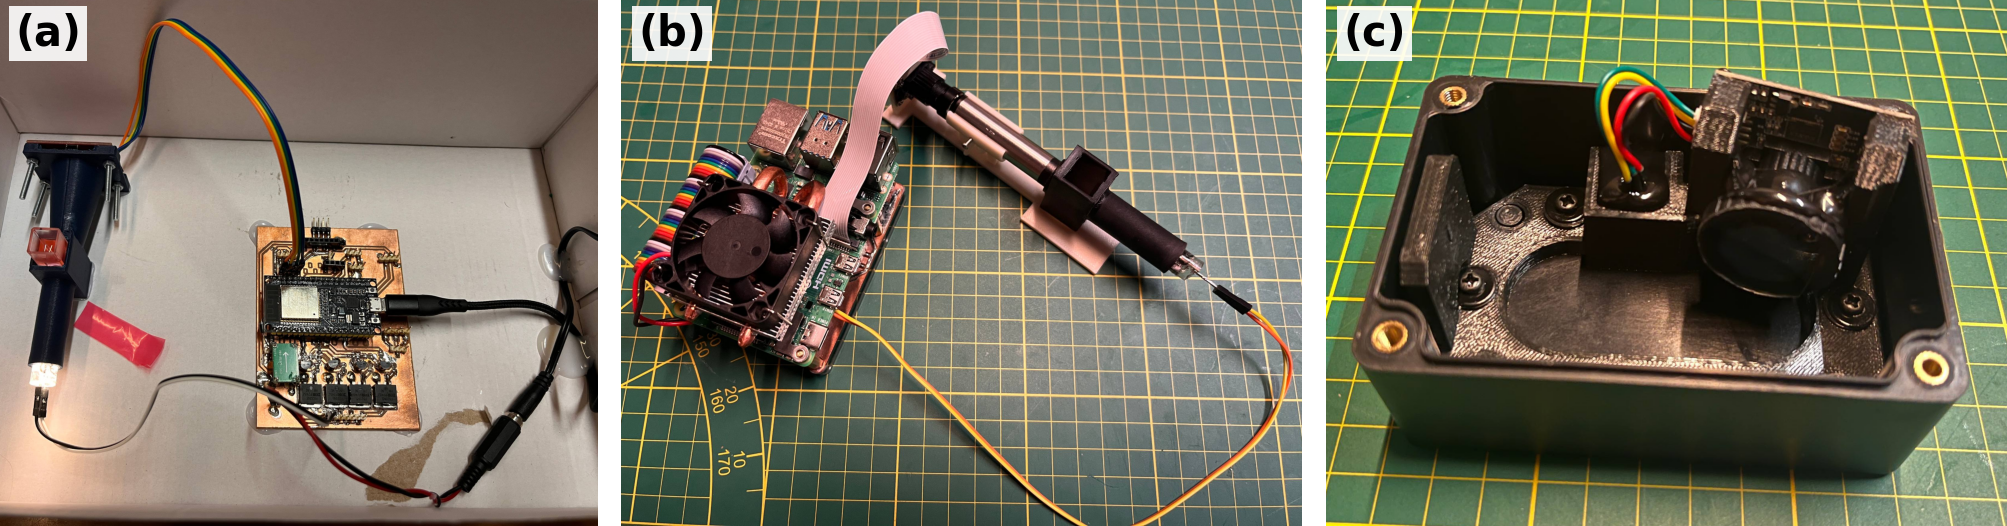
\includegraphics[width=\linewidth, draft=false]{systems.png}

\caption{\FigureCaptionThree}\label{fig:systems}
\end{figure}

System A is built around the SparkFun Triad AS7265x multispectral sensor board (SparkFun Electronics). The board integrates three CMOS devices (AS72651, AS72652, and AS72653; ams OSRAM) and provides 18 spectral channels between 410 and 940~nm. Interference filters deposited on the sensor define the channels, with a nominal FWHM of about 20~nm,\citep{ams2018as7265x} so no external dispersive optics are required. We disabled the built-in LEDs so that the sensor could be used with the external source, and mounted the assembly on a custom 3D-printed structure. An ESP32 microcontroller handled communication and acquisition, and the acquisition software averaged ten consecutive measurements per reading. Absorbance was calculated as the base-10 logarithm of the ratio between blank and sample intensities.

System B is an imaging spectrometer: a Raspberry Pi camera records the output of a commercial pocket spectroscope fitted with a transmission diffraction grating (Pocket Spectroscope, Paton Hawksley Education).\citep{patonPocket} A 12~mm M12 lens focuses the spectrum onto the sensor, and a Raspberry Pi 4B single-board computer (Raspberry Pi Ltd) controls acquisition. Camera and spectroscope were mounted on a custom 3D-printed structure. Spectra were acquired and processed with PySpectrometer2,\citep{wrightPySpectrometer2} which extracts the spectrum by vertical averaging and supports wavelength calibration with several reference points.

System C is the Little Garden spectrometer, a commercial low-cost instrument. Inside a 3D-printed enclosure that connects to a computer by USB, it combines a modified webcam, with the Bayer filter removed to increase sensitivity, and a grating cut from a DVD. Spectra were acquired with the Theremino Spectrometer software\citep{thereminoSpectrometer} at a resolution of 1920\,$\times$\,1080 pixels. Before each measurement, we adjusted the vertical region of interest by hand so as to capture the spectrum while keeping the background low.

The three systems shared the same 10~W halogen lamp, but their holders and collection optics differed, so their complete optical paths were not identical.

\subsubsection{Calibration}\label{subsec2.2}

\paragraph{Preparation of the dye solutions}\label{subsubsec2.2.1}

Each of the eleven solutions contained one drop of a commercial food dye in 10~mL of distilled water (twelve-color set, 6~mL per bottle; Amazon ASIN B08X6FMHKP). The manufacturer does not disclose the colorants or their concentrations, so we identify the dyes by their commercial names and reference spectra. Eight dyes (grape, lemon, lime, navy, orange, pink, rose, and teal) supplied the calibration data, while the blue, green, and red dyes were kept out of fitting and model selection and reserved for validation. Validation therefore concerns new solutions from the same family of colorants, whose absorption bands may overlap (blue and teal both peak near 630~nm). The lemon and rose solutions reached absorbances of 2.85 and 2.68, beyond the range over which the photometric accuracy of the reference is specified; these values were retained in the calibration fits. Nine of the reference spectra are shown in Figure~\ref{fig:dyes}; orange and pink are omitted.

\begin{figure}[!htbp]
\centering
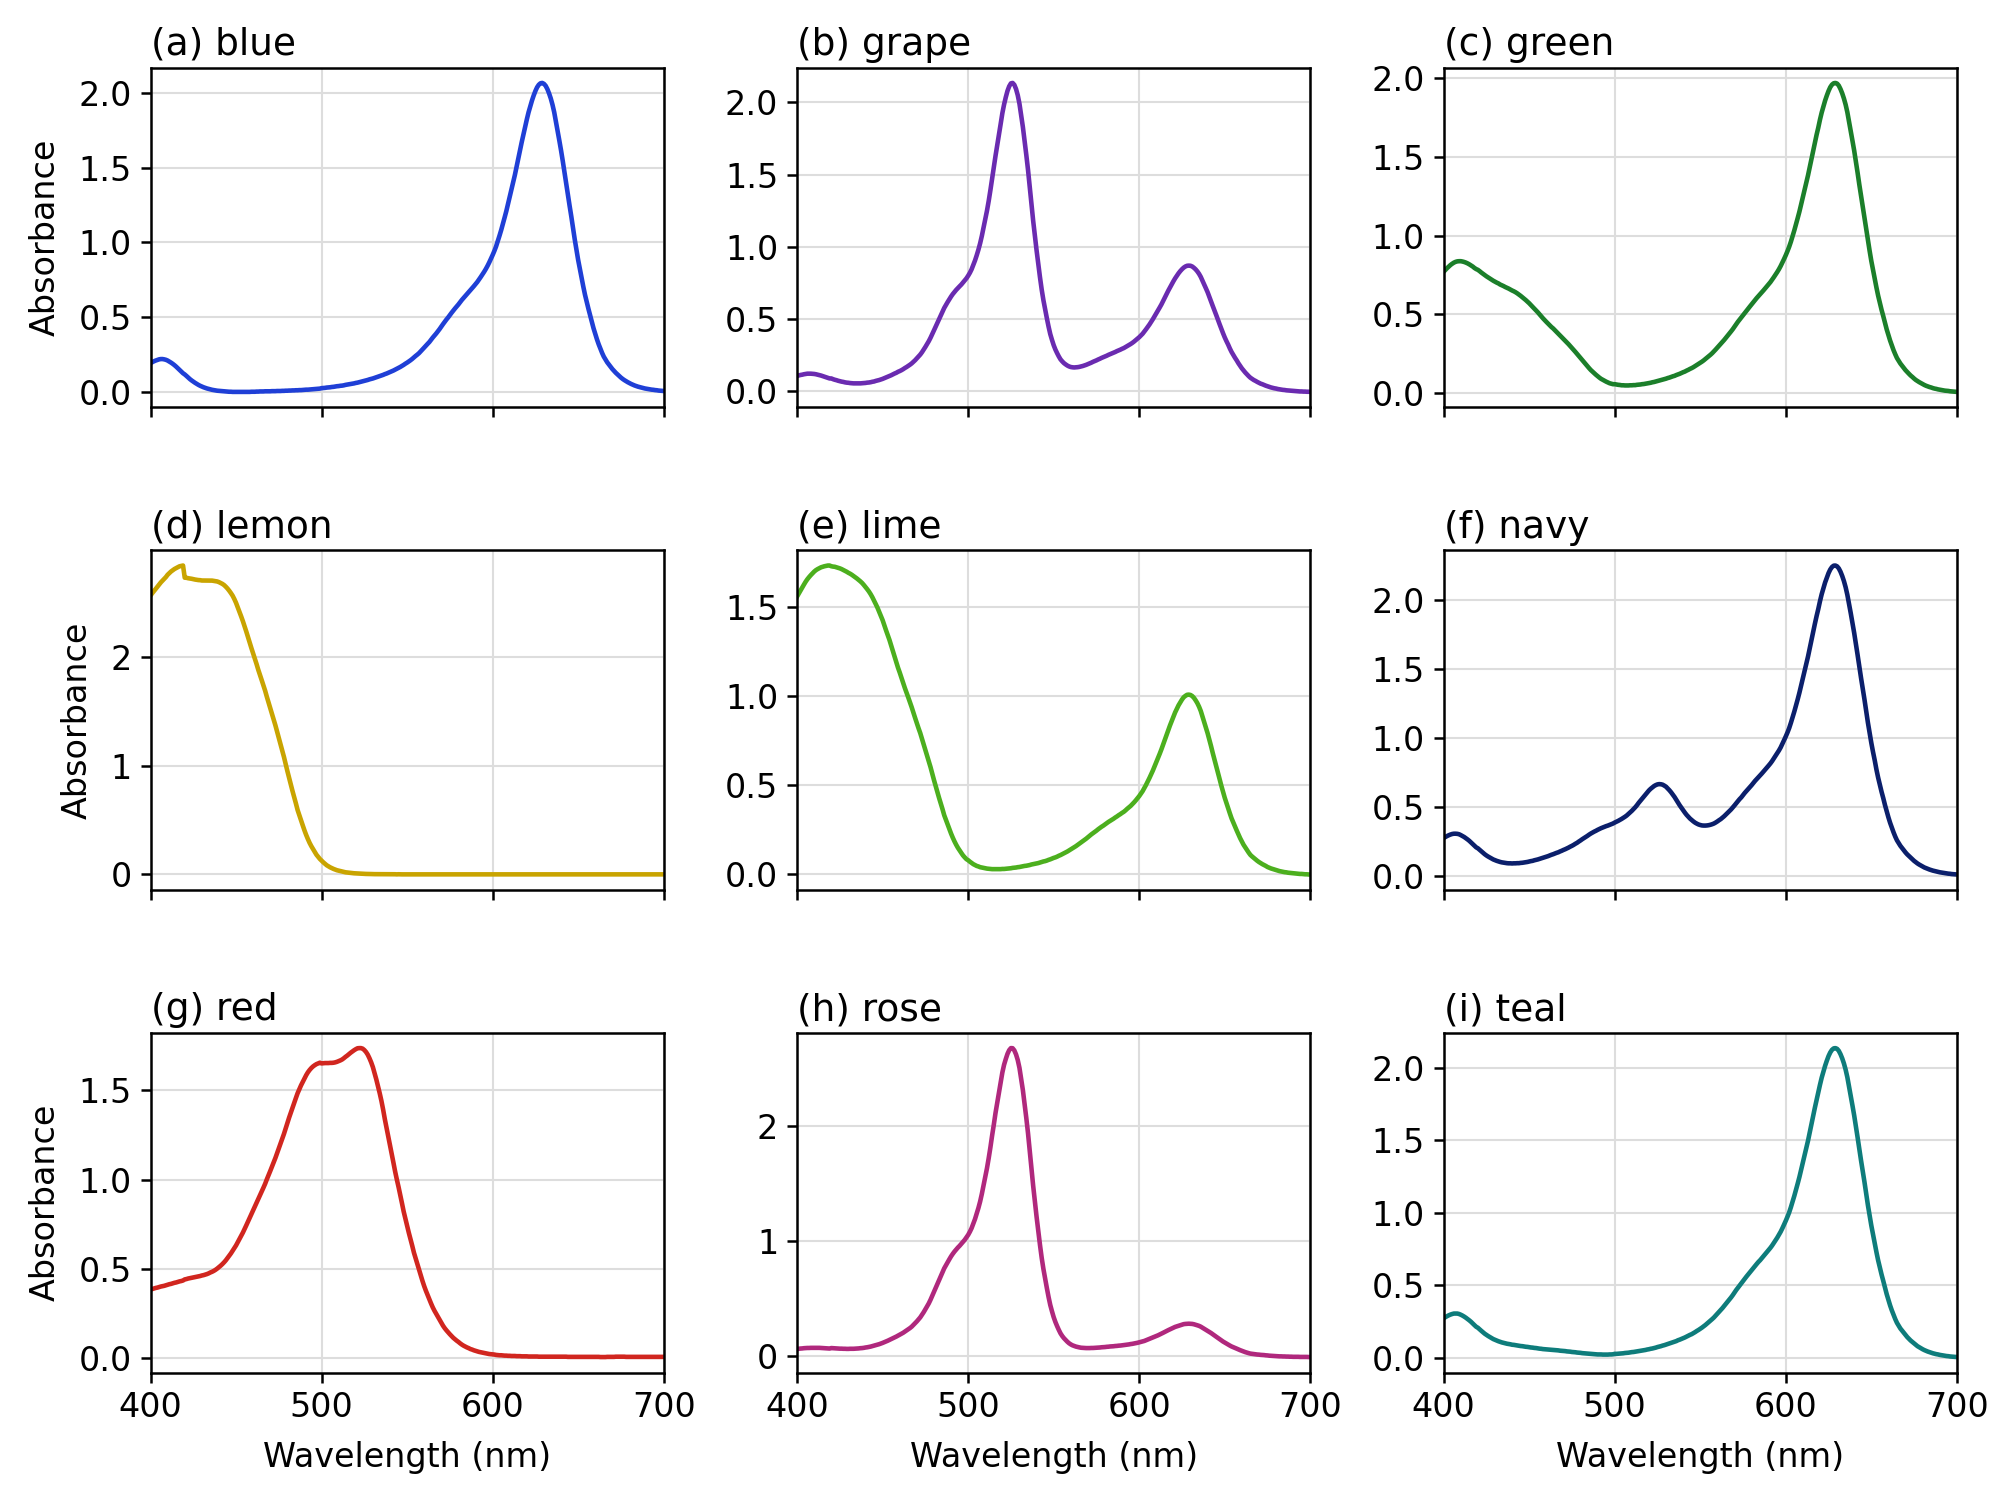
\includegraphics[width=\linewidth, draft=false]{commercial.png}

\caption{\FigureCaptionFour}\label{fig:dyes}
\end{figure}

\paragraph{Wavelength calibration}\label{subsubsec2.2.2}

For system A we relied on the nominal channel centers and did not independently verify the position or response of the channels. For the two imaging systems, mercury lines defined the mapping from pixels to wavelengths: a cubic polynomial through 404.7, 435.8, 546.1, and 577.0~nm for system B, and a straight line through 435.8 and 546.1~nm for system C. A cubic through four points and a line through two leave no residual degrees of freedom, and we did not measure any additional line to check either mapping.

\paragraph{Absorbance calibration}\label{subsubsec2.2.3}

Measured absorbance $s$ was related to reference absorbance $A_{\text{ref}}$ through a wavelength-dependent gain and offset:
\begin{equation}\label{eq:cal}
A_{\text{ref}} \;=\; a_1(\lambda)\, s \;+\; a_0(\lambda)
\end{equation}
where $a_1$ is the gain, $a_0$ the offset, and $\lambda$ the wavelength. Before fitting, measured absorbances above 5 were excluded automatically, and calibration required at least three valid dye pairs at each wavelength. Systems A and C used eight calibration pairs throughout. System B used seven pairs below 420~nm, where the navy dye measurements exceeded the threshold, and eight at the remaining wavelengths. Adding a second-order term in $s$ to Eq.~\ref{eq:cal} did not improve leave-one-dye-out prediction within the eight calibration dyes and was unstable for system B, so we kept the first-order model.

A single gain and offset for all wavelengths could not reproduce the reference. For systems B and C, we therefore expanded $a_1(\lambda)$ and $a_0(\lambda)$ in an orthogonal polynomial basis of normalized wavelength, of degree 18 for B and 8 for C, and fitted them jointly by least squares across all calibration dyes and wavelengths. Both degrees were selected by leave-one-dye-out cross-validation within the eight calibration dyes, so the validation dyes stayed outside model selection. The resulting smooth surfaces can be evaluated anywhere in the calibrated range. The discrete channels of system A were fitted separately, with two coefficients per channel, whereas systems B and C need two coefficients per term of the polynomial expansion.

\subsubsection{Validation measurements and metrics}\label{subsec2.3}

All measurements were made in 10~mm plastic cuvettes, in darkness and at an ambient temperature of 22~$^\circ$C, with blank and dark spectra acquired before each series. Each validation dye was measured 100 times on each system, with the cuvette repositioned by hand between readings.

To summarize agreement over 400--700~nm, we used the root-mean-square difference (RMSD), pooling the paired differences between calibrated and reference absorbance over all wavelengths and the three validation dyes. The squared Pearson correlation ($r^2$) was computed separately for each dye and then averaged. RMSD measures differences in absorbance units, whereas $r^2$ captures how well the spectral shapes match and is insensitive to a constant bias. System A was compared with the reference at its nominal channel centers, and systems B and C on their own wavelength grids.

For repeatability, we computed the SD of the 100 readings at each wavelength and averaged it over wavelength and over the three dyes. The pointwise coefficient of variation was $\mathrm{CV}=100\,\mathrm{SD}/\overline{A}$, where $\overline{A}$ is the mean absorbance, using only points with $\overline{A}>0.05$; these CVs were averaged over wavelength for each dye and then over the three dyes. SD thus expresses absolute dispersion, and CV dispersion relative to the mean signal. Since each reading of system A is already an average of ten sensor measurements, the repeatability results describe the acquisition procedures as they were used. We did not quantify spectral resolution, portability, ease of use, assembly time, maintenance effort, or power demand.
\FloatBarrier

\subsection{Results and discussion}\label{sec4}

Table~\ref{tab:metrics} summarizes, for each system, the agreement with the reference (RMSD and $r^2$), the spectral sampling ($n_\lambda$, the number of wavelengths per dye), the size of the calibration ($N_c$, the total number of fitted coefficients), and the repeatability (SD and CV), all over 400--700~nm and the three validation dyes. The pooled comparisons contain 33, 903, and 1710 wavelength--dye pairs for systems A, B, and C; because neighboring spectral points are correlated, these numbers are not counts of independent samples.

Of the three, system B came closest to the reference in absorbance and had the smallest absolute SD. System C had a slightly higher RMSD and greater dispersion, but needed the fewest calibration coefficients.

\begin{table}[!htbp]
\doublespacing
\caption{Performance of systems A, B, and C on the three validation dyes over 400--700~nm}\label{tab:metrics}
\centering

\begin{tabular}{lrrrrrr}
\toprule
System & RMSD & $r^{2}$ & $n_\lambda$ & $N_{c}$ & SD & CV (\%) \\
\midrule
A & 0.281 & 0.805 & 11  & 22 & 0.050 & 12.1 \\
B & 0.077 & 0.983 & 301 & 38 & 0.032 & 11.1 \\
C & 0.094 & 0.975 & 570 & 18 & 0.086 & 32.3 \\
\bottomrule
\end{tabular}

\end{table}

\begin{figure}[!htbp]
\centering
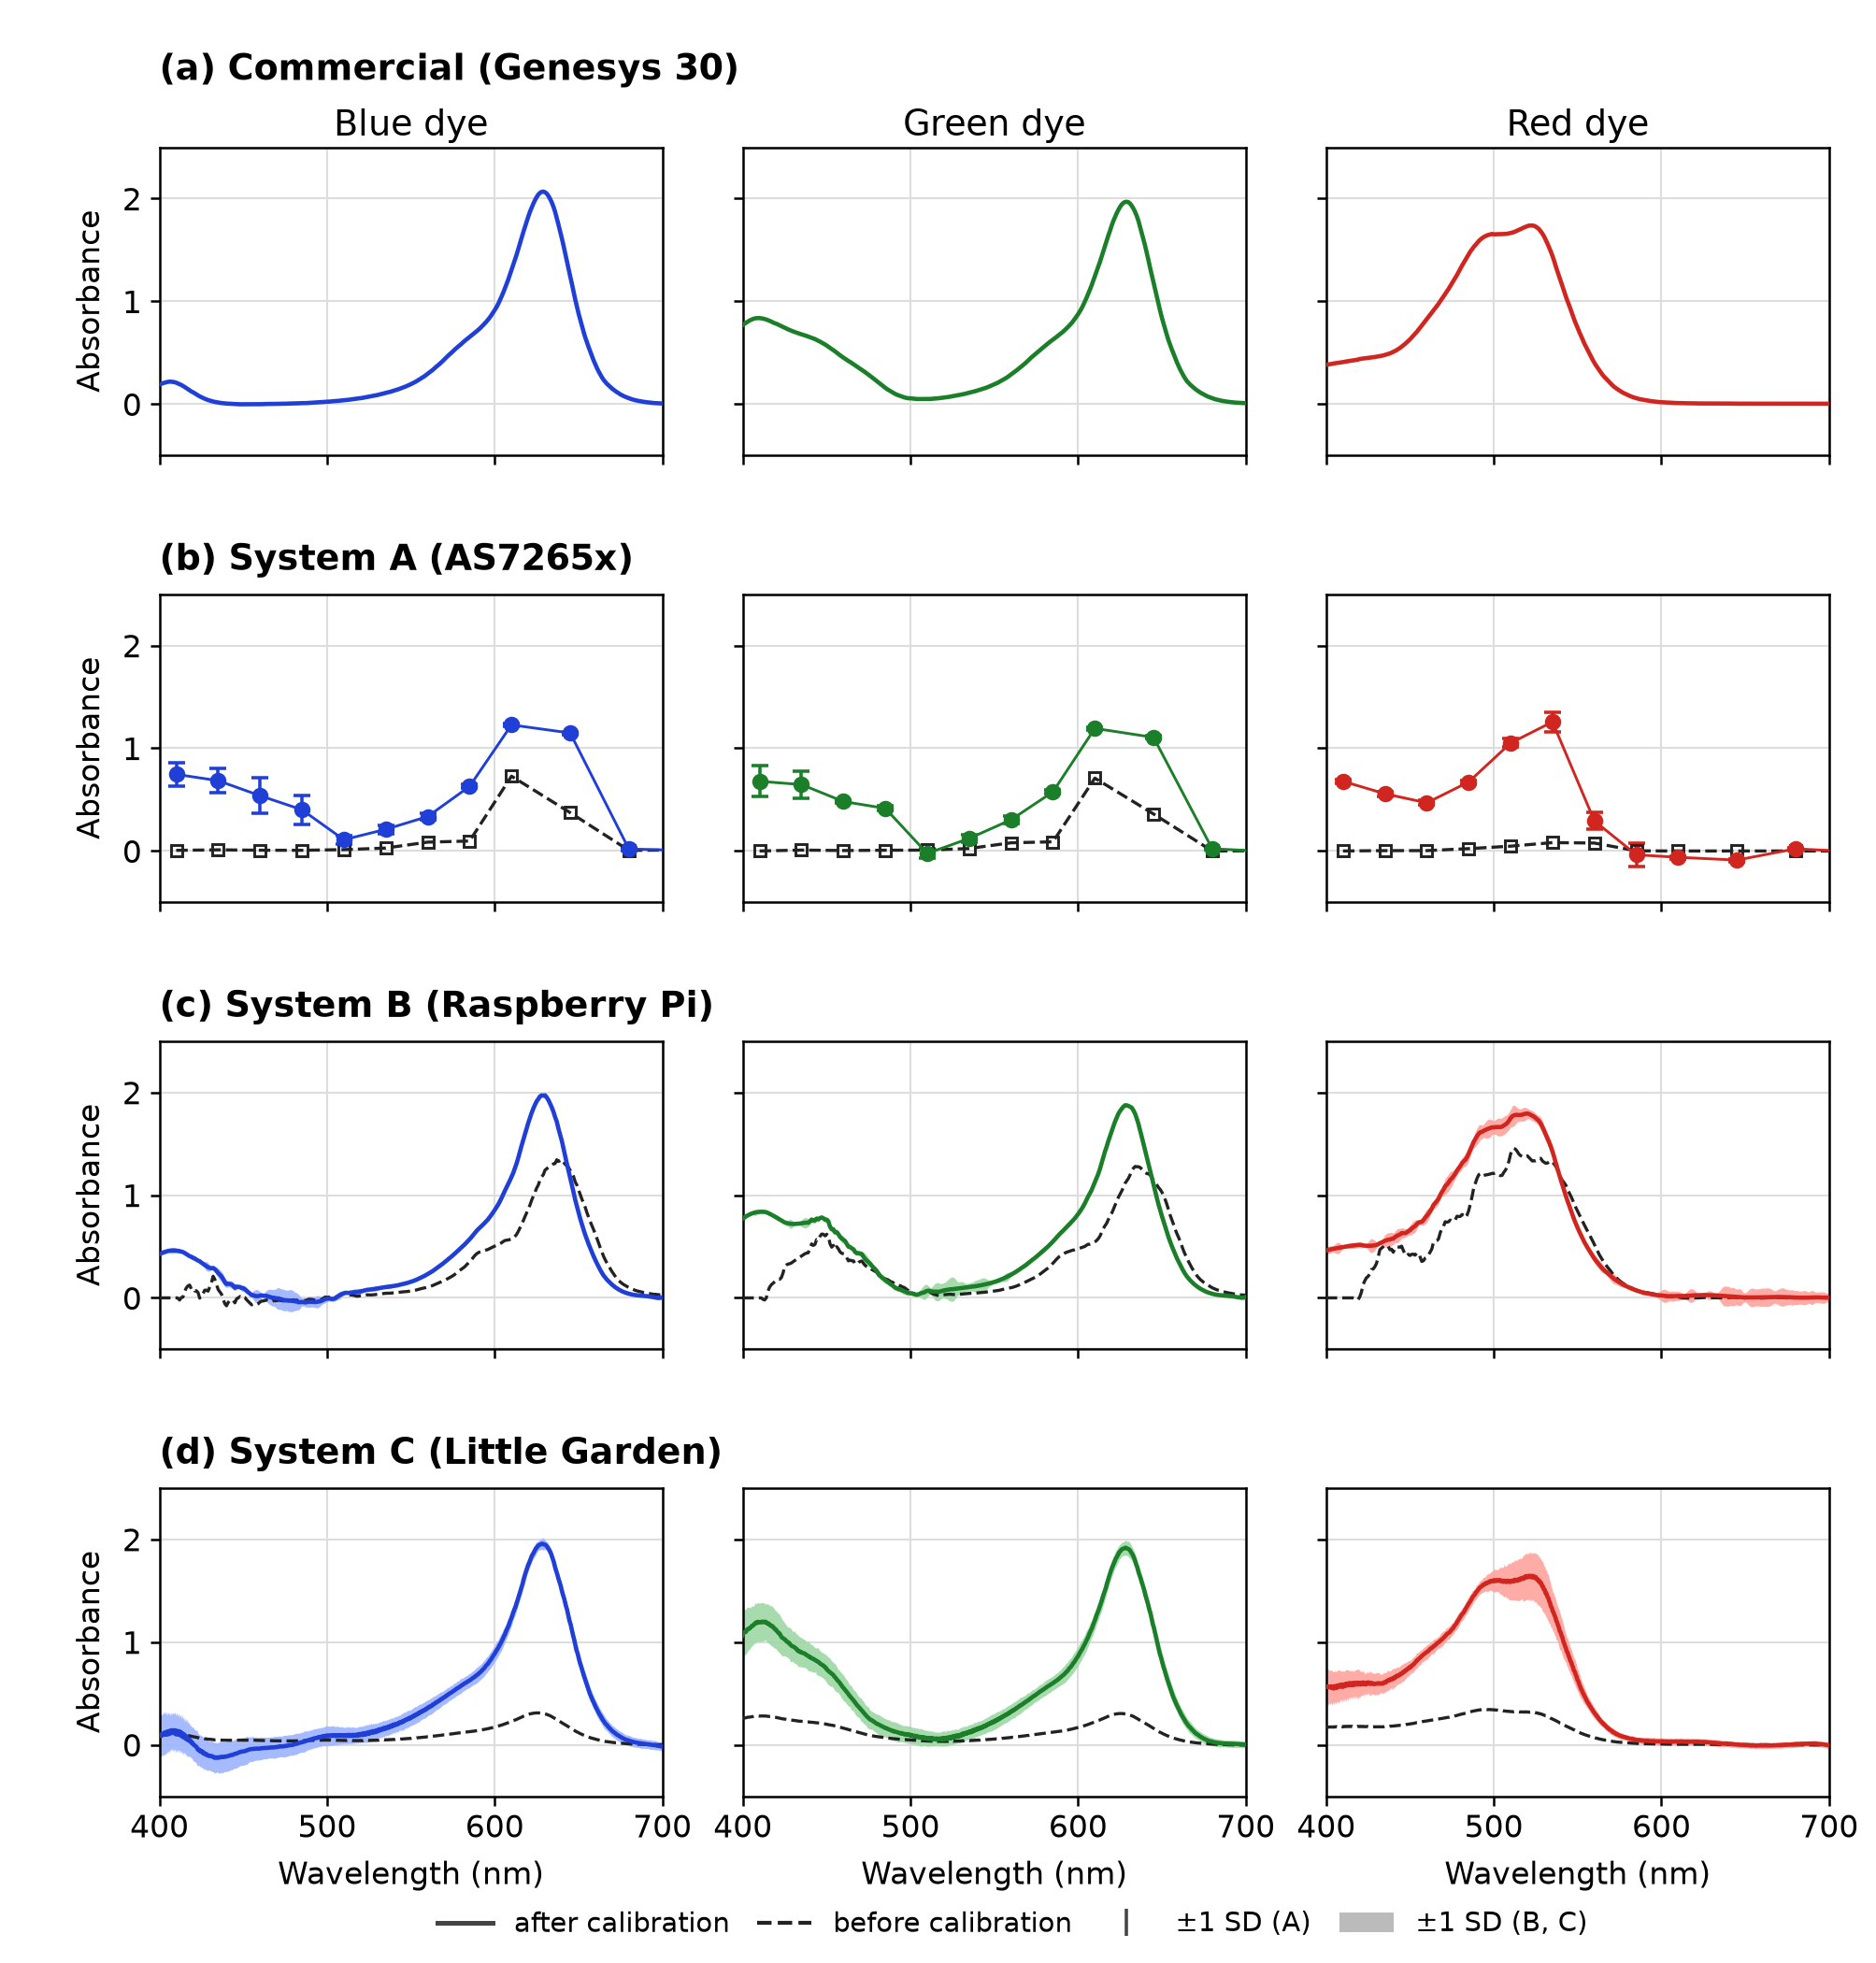
\includegraphics[width=\linewidth, draft=false]{comparison.png}

\caption{\FigureCaptionFive}\label{fig:comparison}
\end{figure}
\FloatBarrier


All three systems located the main absorption bands (Figure~\ref{fig:comparison}). Calibration stretched the initially compressed responses, above all those of systems A and C; such compression is consistent with stray light and with broad effective bandwidths, neither of which we measured. System A captured the overall shape of the spectra but missed their finer detail, while system B showed moderate noise in the blue region and weaker noise in the green. The wider shaded bands of system C reflect its larger absolute SD. Both channel bandwidth and optical coupling affect how system A compares with point values of the reference, but we were unable to separate their contributions.

In Figure~\ref{fig:map}, the points for systems B and C lie close to the identity line over most of the range, while those for system A scatter more widely. Below 480~nm, the mean absolute differences were 2.1, 2.3, and 3.4 times larger than above 480~nm for systems A, B, and C, respectively. This pattern is consistent with the weak blue output of the halogen lamp, but since the three systems share silicon detectors, cuvettes, and calibration samples, we could not isolate its contribution.

\begin{figure}[!htbp]
\centering
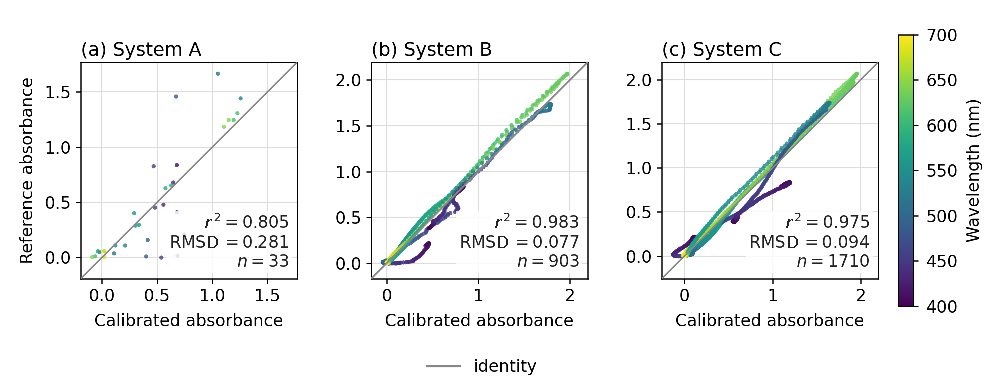
\includegraphics[width=\linewidth, draft=false]{dispersion.pdf}

\caption{\FigureCaptionSix}\label{fig:map}
\end{figure}

\subsubsection{Implementation and cost}\label{sec4.1}

System A cost \euro{}88: \euro{}65 for the sensor, \euro{}8 for the controller, \euro{}10 for the enclosure and accessories, and \euro{}5 for wiring, circuit board, and power supply. System B cost \euro{}215: \euro{}15 for the camera, \euro{}65 for the Raspberry Pi, \euro{}15 for the lens, \euro{}100 for the spectroscope, \euro{}10 for the enclosure and accessories, and \euro{}10 for wiring, circuit board, and power supply. System C was bought as a complete retail instrument for \euro{}90. None of these totals includes the shared halogen lamp, the purchase dates are not available, and the component totals for systems A and B do not cover the same items as the retail price of system C.

\subsubsection{Scope and limitations}\label{sec:caselim}

Our comparison rests on a single unit of each system and on three validation solutions from the same family of colorants as the calibration set, and two of the calibration dyes exceeded the specified photometric range of the reference. We did not measure resolution, stray light, drift, transfer between units, performance in real matrices, or detection limits. Neither the nominal filter responses nor the wavelength mappings were verified independently, and the systems are no longer available for further measurements. The results therefore apply to the units, calibrations, and acquisition settings we tested.
\FloatBarrier
